\documentclass[authordate, empirical]{jote-new-article}

\usepackage{caption}

\usepackage{tabularx}

\usepackage{graphicx}

\usepackage{hyperref}

\usepackage[backend=biber,style=apa]{biblatex}

\addbibresource{bibliography.bib}

\jotetitle{Some Data Indicating that Editors and Reviewers Do Not Check Preregistrations during the Review Process}
\keywordsabstract{Preregistration, Pre-registration, Trial Registration, meta-science, Open Science}
\abstracttext{If a study is preregistered, but nobody checks it during review, does it mean anything? The purpose of this preregistered study was to better understand how editors and reviewers engage with preregistration plans during the review process. The article set was retrieved from the \emph{PLOS} family of journals, which a) are cross-disciplinary, b) are open access, c) have a relatively high frequency of preregistered studies, and d) most importantly, in 2019 began publishing manuscript reviews alongside published articles. A total of 693 articles were identified via the initial search, which was reduced to 201 that met the review criteria. For each article, the review history was coded for whether editors or reviewers a) mentioned the preregistration, b) accessed the preregistration, and c) made specific mention of the relation between the preregistration and reporting in the paper. Analyses were conducted at the article level (i.e., did any reviewer or editor mention/access/compare; n = 201) and the editor/reviewer level (i.e., overall, how many editors/reviewers mention/access/compare; \emph{n} = 689). At the article level, for 43\% of articles at least one editor/reviewer mentioned the preregistration, but in only 14\% did they mention accessing the preregistration and in 10\% did someone make a clear statement about the relation between the preregistration and the manuscript. In contrast, at the editor/reviewer level things looked much worse, with only 18\% mentioning preregistration, 5\% reporting accessing the preregistration, and 3\% discussing the relation between the preregistration and the manuscript. These data suggest very low levels of engagement with preregistrations during the review process, which undermines some of the primary goals of the practice. }
\runningauthor{Syed}
\jname{Journal of Trial \& Error}
\jyear{2025}
\paperdoi{10.36850/e5ce-4cc5}
\paperreceived{August 1, 2024}
\author[1]{\mbox{Moin Syed\orcid{0000-0003-4759-3555}}}
\affil[1]{University of Minnesota}
\corremail{\href{mailto:moin@umn.edu}{moin@umn.edu}}
\corraddress{University of Minnesota}
\runningauthor{Syed}
\paperaccepted{January 18, 2025}
\paperpublished{March 1, 2025}
\paperpublisheddate{2025-03-01}
\jwebsite{https://journal.trialanderror.org}

\begin{document}
\begin{frontmatter}
  \maketitle
  \begin{abstract}
    \printabstracttext
  \end{abstract}
\end{frontmatter}





	\section{\textbf{Introduction}}



	Preregistration refers to the process of formally documenting study design and/or analysis plans prior to implementation (Nosek et al., 2018; Wagenmakers et al., 2012). Although registration of clinical trials has been a long-standing practice, the preregistration movement pioneered in psychology sought to bring greater depth and detail to the study planning process (Thibault et al., 2023). Examples and templates for preregistrations are now available for a wide variety of study designs and contexts, including experiments (van 't Veer \& Giner-Sorolla, 2016), secondary data (van den Akker et al., 2021), meta-analyses (Quintana, 2015), and qualitative methods (Haven \& Van Grootel, 2019), and has expanded from psychology to a wide variety of biological research topics and methods (Conix et al., 2023; Dirnagl, 2020; Errington et al., 2021; Pariente, 2022).



	As preregistration has become increasingly prominent (Nosek et al., 2018) it has also been subject to criticism (e.g., Szollosi et al., 2020; see Syed, 2024). Moreover, despite the fact that researchers generally have positive attitudes and see many benefits to preregistration, they also identify barriers to implementation (Spitzer \& Mueller, 2023). Scrutiny of widely promoted and adopted practices is crucial for successful implementation and ensuring that practices achieve their intended goal. The purpose of the present study is aligned with this aim by examining how editors and peer reviewers interact with preregistrations during the review process.



	\section{\textbf{Background and rationale}}



	Multiple rationales for why preregistration is beneficial have been advanced, including that it helps distinguish between data-independent and data-dependent tests, reduces the opportunity for questionable research practices, facilitates conducting severe tests of hypotheses, and that it increases the thoughtfulness and planning of research projects (Lakens, 2019; Nosek et al., 2018; Syed, 2024; Wagenmakers et al., 2012). Criticisms and limitations of preregistration have also been identified, including that it may lead to overvaluing pre-planned analyses at the expense of exploratory, emergent findings (Rubin \& Donkin, 2022), that it does not contribute to theoretical developments (Szollosi et al., 2020), and that it does not serve as a marker of study quality (Schneider et al., 2022).



	The introduction of “badges” affixed to articles that include preregistered studies seems to signal that preregistration is, \emph{prima facie,} a marker of study quality (Kidwell et al., 2016; Schneider et al., 2022). This is, unfortunately, not the case for both procedural and substantive reasons. Procedurally, an article can receive a preregistration badge even if only one of multiple studies reported therein was preregistered. Moreover, preregistration plans can vary in their scope and specificity, ranging from vague descriptions of research questions and hypotheses to the inclusion of analytic scripts prepared based on synthetic data (Thibault et al., 2023). More critically, however, is that the substantive nature of preregistrations is such that they are only informative of the degree of \emph{transparency} exhibited by researchers and not all about the \emph{credibility} of the study results. That is, preregistrations potentially provide insight into the plans and intentions of researchers before conducting a study and/or analyzing the data, but they do not, on their own, speak to the value, reliability, or rigor of the findings of the study. This distinction is not meant to minimize the value of transparency—indeed, transparency is a precondition for credibility (Vazire, 2017)—but rather to be clear on what is and is not the scientific value of preregistration.



	That preregistration is not an indicator of credibility has been revealed through recent meta-scientific research on the practice. Preregistrations are the \emph{plans}, what the researchers intended to do prior to working with their data. The map, however, is not the territory, and thus these plans do not necessarily correspond to what was actually reported in the final articles. Studies comparing preregistration plans to reporting in the corresponding articles have found evidence of substantial discrepancies, including selective hypothesis reporting, changes in the analysis, and changes in exclusion criteria (Claesen et al., 2021; van den Akker et al., 2023). These kinds of problems have been long-known in the context of trial registrations, in which there is a high rate of primary outcome switching (Kampman et al., 2022). Accordingly, just because a study is preregistered does not mean that the researchers closely followed their pre-specified plans.



	Of course, deviating from a preregistration plan is not an inherently bad practice. Researchers do not have perfect foresight and often make mistakes. It is always a better choice to conduct the most sensible analysis rather than sticking with a weaker analysis just because it was prespecified (Lakens, 2024). The principle of transparency, however, should be carried through, and any deviations from the preregistration plan should be transparently reported in the manuscript (see Willroth \& Atherton, 2024, for an excellent guide on how to handle deviations). Moreover, any preregistered analyses that are no longer primary should still be reported, perhaps in the supplemental files, which then allows readers to evaluate the credibility of the deviations.



	The high rate of discrepancies between preregistration plans and reporting in articles suggests that the plans may not be frequently evaluated during the peer review process. Data on editors' and reviewers' self-reports of their tendency to review preregistration plans suggested an average rate of 65\% for both (Willroth \& Atherton, 2024). However, they relied on a select sample and retrospective averaged reporting. A more representative, yet still retrospective, analysis of reviewers' and authors' reports of checking trial registrations during the review process, found a lower rate of 34\% (Mathieu, 2009). The retrospective self-report approach taken in both of these studies is limited in comparison to examining actual verifiable behaviors.



	The purpose of the present study was to examine how editors and peer reviewers interact with preregistrations during the review process. An ostensible role of peer reviewers evaluating manuscripts with preregistered studies would be to ensure transparency in deviations by comparing the manuscript to the preregistration plan. There are two reasons to doubt that this occurs with high frequency. First, is the aforementioned research on the high rates of deviations. Second is my own personal experience as an editor and reviewer, in which I not only frequently observe substantial undisclosed deviations from preregistration plans, but also typically am typically the only editor/reviewer to report even accessing the preregistration plan, let alone evaluating the manuscript against it. Indeed, the impetus for this entire project was a review that I conducted for an ostensibly leading journal in psychology where the study was reportedly preregistered, but the manuscript included substantial undisclosed deviations that raised serious questions about the work. Because this was not the first time I had such an experience, I decided to act on my frustration with the failure to disclose deviations from preregistrations and investigate the phenomenon empirically..



	The current study examined the following preregistered (\url{https://osf.io/ma37t}) research questions:

	\begin{enumerate}


		\item How often do editors and reviewers mention preregistration during the review process?



		\item
		When editors and reviewers do mention the preregistration, how do they characterize it (e.g., positively, neutrally, negatively)?



		\item How often do editors and reviewers report accessing the preregistration plans?



		\item
		How often do editors and reviewers report on the relation between the preregistration plans and reporting in the article? When they do, what do they highlight?



		\item Are there any variations in the preceding by discipline, journal, or research topic?


	\end{enumerate}

	\section{\textbf{Method}}



	\subsection{Article selection}



	The current project required a set of articles that a) were preregistered and b) have open peer review history, which would then allow for an examination of editors/reviewers discussing the preregistration during the review process. For this reason, the \emph{PLOS} family of journals was selected as the target for the analysis. \emph{PLOS} journals not only promote preregistration and (as of May 2019) publish the review history alongside their articles, but they publish a large volume of articles, which suggested that there would be a sufficient set for analysis. An additional positive feature is that all articles are open access, so any researchers interested in building upon the current study will have access to do so. Clearly, there are other journals that could be included, but this project was intended to be a relatively small-scale initial study to understand how editors/reviewers engage with preregistrations during the review process.



	The article search process was conducted prior to the study registration to ensure there was a sufficient number of articles to be analyzed. The search string,



	((everything:preregist*) OR everything:pre-regist*)



	was entered into the \emph{PLOS} search tool,\url{https://journals.plos.org/plosone/search}, on October 27, 2023, yielding 693 articles. Although \emph{PLOS} did not begin publishing article review histories until May 2019, to be maximally inclusive no specific date restrictions were set on the search. There was no \emph{a priori} definition of a “sufficient” number of articles and I did not conduct a power analysis (no inferential statistics are involved in this study). Rather, I simply estimated the result to determine whether it was likely to lead to a reasonable number of articles that could be analyzed, and decided that it was. Although the search tool is based within the \emph{PLOS ONE} site, it searches all \emph{PLOS} journals. To confirm this, I ran the same search from the \emph{PLOS Biology} search tool and got the same results. The results were exported to Zotero using the Zotero Connector Chrome extension. No further analysis was conducted prior to the registration.



	It is worth noting that the search string would not necessarily discover trial registrations, which may not use the language of “preregistration.” This is acceptable because the study is focused on preregistration specifically, which often involves a more elaborated study and analysis plan than do trial registrations. Nevertheless, trial registrations that were included in the final article set were analyzed.



	\subsection{Inclusion and exclusion criteria}



	There were three requirements to be included in the analysis: 1) the article must indicate that at least one study reported therein was preregistered, 2) the article peer review history must be available, and 3) it must be an empirical article (quantitative, qualitative, or mixed methods), including meta-analyses. Narrative reviews, commentaries, and methodological papers were screened out.



	The only exclusion criterion was that Registered Reports (Chambers \& Tzavella, 2021) were not included in the analysis. Because the Stage 1 manuscript is essentially the preregistration plan for that article format, the reviewers will have necessarily examined and commented on it. Of course, the Stage 2 manuscript could be reviewed by different people from the Stage 1, and even the same reviewers will not necessarily compare the Stage 2 to Stage 1, but nevertheless, they were excluded.



	\subsection{Article coding}



	I conducted all article screening, beginning with whether or not the review reports were openly available, as this was quick and easy to ascertain. I then coded all of the included articles for the specific features of interest. A random sample of 20\% of articles were checked by reliability coders who were unaware of my coding. Reliability was assessed using percent agreement, set at a threshold of 80\%, which is appropriate given the likelihood of highly skewed marginal distributions (see Syed \& Nelson, 2015). Percent agreement for all coding categories exceeded the 80\% threshold.



	Each included article was coded for the elements noted below. All rounds of review were examined (i.e., every available decision letter), but coding was collapsed across rounds. There was no coding system specified for discipline, journal, or keywords (to address Research Question 5), as these data were to be drawn directly from the article meta-data.



	\subsection{Editor/Reviewer mentions preregistration in their reviews}



	Each editor/reviewer for which there is an open report received a simple Yes/No as to whether they mentioned the preregistration at all.



	\subsection{Editor/Reviewer's characterization of preregistration}



	For those who did reference the preregistration, a brief description of the characterization was noted. The initial expectation was that these would be coded as positive (e.g., “It is great to see that the study was preregistered”), neutral (e.g., “This study was preregistered”), or negative (e.g., “Unfortunately, the preregistration led the authors stick with poor analytic choices.”), but I also allowed room for additional or alternative characterizations (there weren't any).



	\subsection{Editor/Reviewer indicates accessing the preregistration }



	For those who did reference the preregistration, a Yes/No code was assigned as to whether they made any statement that indicated that they accessed, attempted to access, and/or reviewed the preregistration as part of the review process.



	\subsection{Editor/Reviewer comments on the relation between the preregistration and the manuscript}



	For those who did reference accessing the registration, a Yes/No code was assigned as to whether they made any specific statements about the relation between the registration and what is reported in the article. A follow-up open-ended code briefly summarized the nature of the comment.



	\section{Results}



	The study preregistration (\url{https://osf.io/ma37t}) was submitted following the initial article search, and all reported analyses were preregistered unless otherwise specified. Data, analysis code, and study materials are available at \url{https://osf.io/nmhbf/}. Analyses were conducted in R v.4.3.1 (R Core Team, 2022) via RStudio v.2023.09.1 (Posit Team, 2023), with support from the \emph{dplyr} (Wickham et al., 2023), \emph{tidyr }(Wickham et al., 2023), \emph{summarytools }(Comtois, 2022), \emph{ggplot2 }(Wickham, 2016), and \emph{cowplot }(Wilke, 2020) packages.

	\begin{figure}
		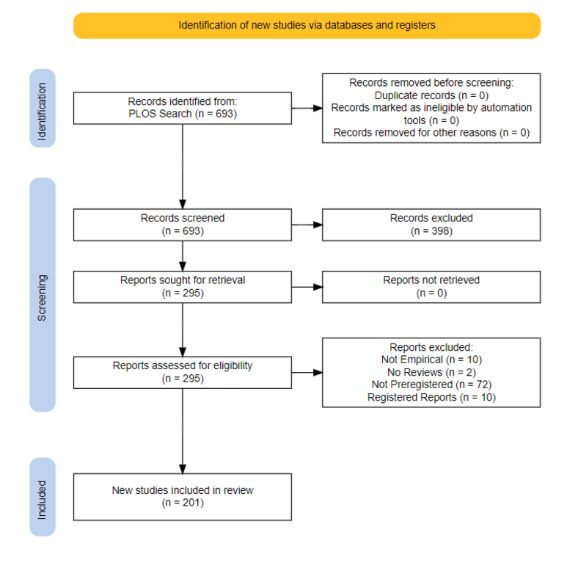
\includegraphics[width=\linewidth]{media/image1.png}

		\caption{\textbf{PRISMA diagram illustrating the article search and screening process.} Created using the Shiny App developed by Haddaway et al. (2022).}

		\label{fig:rId8}


	\end{figure}


	As noted, the initial search resulted in 693 articles, of which 295 (43\%) had open peer review history. Article screening for inclusion and exclusion criteria led to the removal of 10 articles that were not empirical, an additional 2 that ended up not having the review history, an additional 72 that were not preregistered, and an additional 10 that were Registered Reports. This led to a final analytic sample of 201 articles (Fig 1). All articles had at least one reviewer in addition to the editor, with 6.5\% having only one reviewer, 58\% having two, 25\% with three, 9\% with four, 1.5\% with five, and just one article with six (\emph{M} = 2.43, \emph{SD} = 0.84). Because the analyses here were not intended to distinguish between editor and reviewer comments, they were all collapsed together into a single editor/reviewer category, and thus the average number of people who reviewed each article was 3.43 (\emph{SD} = 0.84) with a mode of 3. The rationale for collapsing editors and reviewers together was that my primary interest in this project was whether evaluators were engaging with the preregistrations, and not who specifically was doing so. Nevertheless, because it could certainly be useful to understand differences in behavior between editors and reviewers, the Results section includes some unregistered exploratory analyses on the comparison.

	

	The majority of included articles were published in \emph{PLOS ONE} (82\%), followed by \emph{PLOS Medicine} (9.5\%), \emph{PLOS Computational Biology} (5\%), and \emph{PLOS Biology} (2.5\%), with one each from \emph{PLOS Climate}, \emph{PLOS Digital Health}, and \emph{PLOS Global Public Health}. Analysis of the keywords associated with the articles indicated a wide array of subjects, primarily within the psychological, medical, and biological sciences (see Table 1 for the most frequent keywords and S1 Table for the full list, \url{https://osf.io/p62gh}). With the exception of 2019 (\emph{n} = 4)—the year open peer reviews were initiated at \emph{PLOS} journals—the publication dates were evenly spaced over the years (2020, \emph{n} = 40; 2021, \emph{n} = 57; 2022, \emph{n}= 51; 2023, \emph{n} = 49).



	\begin{table}
		\centering
		\begin{fullwidth}
			\caption{Keywords for Articles Included in Analysis\\ (Frequencies of 10 or greater)}
			\begin{tabularx}{\linewidth}{@{} l X X @{}}
				\toprule
				\textbf{Keyword} & \textbf{Frequency} & \textbf{Percent} \\
				\midrule
				COVID-19 & 35 & 2.18 \\
				Medical risk factors & 31 & 1.93 \\
				Behavior & 29 & 1.80 \\
				Pandemics & 29 & 1.80 \\
				Emotions & 28 & 1.74 \\
				Psychological attitudes & 25 & 1.55 \\
				Decision making & 24 & 1.49 \\
				Surveys & 23 & 1.43 \\
				Metaanalysis & 21 & 1.31 \\
				Human learning & 18 & 1.12 \\
				Sensory perception & 17 & 1.06 \\
				Depression & 15 & 0.93 \\
				Mental health and psychiatry & 15 & 0.93 \\
				Motivation & 14 & 0.87 \\
				Vision & 14 & 0.87 \\
				Children & 13 & 0.81 \\
				Learning & 13 & 0.81 \\
				Virus testing & 13 & 0.81 \\
				Cognition & 12 & 0.75 \\
				Randomized controlled trials & 12 & 0.75 \\
				Systematic reviews & 12 & 0.75 \\
				Food & 11 & 0.68 \\
				Language & 11 & 0.68 \\
				Psychological stress & 10 & 0.62 \\
				Questionnaires & 10 & 0.62 \\
				Reaction time & 10 & 0.62 \\
				Vaccines & 10 & 0.62 \\
				\bottomrule
				\multicolumn{3}{l}{Total \emph{N} for keywords = 1608.  Full list is in S1 Table.} \\
				
			\end{tabularx}
		\end{fullwidth}
	\end{table}
	





	One important analytic decision that was not included in the preregistration was the level at which analyses would be conducted. Because the reviews of each editor/reviewer for each article were coded, analyses could be conducted at the article level (i.e., did any reviewer or editor mention/access/compare; \emph{n} = 201) or at the editor/reviewer level (i.e., overall, how many editors/reviewers mention/access/compare; \emph{n} = 689). Ultimately, I decided both were valuable and provide different types of information, so I am reporting analyses at both levels throughout. All relevant information is included in Fig 2, but below I provide details with respect to the relation between the observed data and the research questions.



	\subsection{How often do editors and reviewers mention preregistration during the review process? When they do, how do they characterize it?}



	In 43\% of articles (\emph{n} = 87), at least one editor/reviewer mentioned the preregistration. For most of these (\emph{n} = 58, 29\% of all articles) only one person mentioned the preregistration, followed by \emph{n} = 23 (11.5\%) for two people, \emph{n} = 5 (2.5\%) for three people, and only one article in which four people mentioned it. Whereas for 43\% of articles at least one editor/reviewer mentioned the preregistration, overall only 18\% of editors/reviewers mentioned the preregistration in their reviews. =The characterization of the mentions was only analyzed at the editor/reviewer level, in which they were mostly positive (59\%), followed by neutral (33\%), and then negative (8\%).

	

	\subsection{How often do editors and reviewers report accessing the preregistration plans?}



	In 14\% of articles (\emph{n} = 28) at least one editor/reviewer reported accessing and/or reviewing the preregistration (one person: \emph{n} = 23, 11.5\%; two people: \emph{n} = 5, 2.5\%), but this frequency dropped to just 5\% when looking at the editor/reviewer level.


	\begin{figure*}
		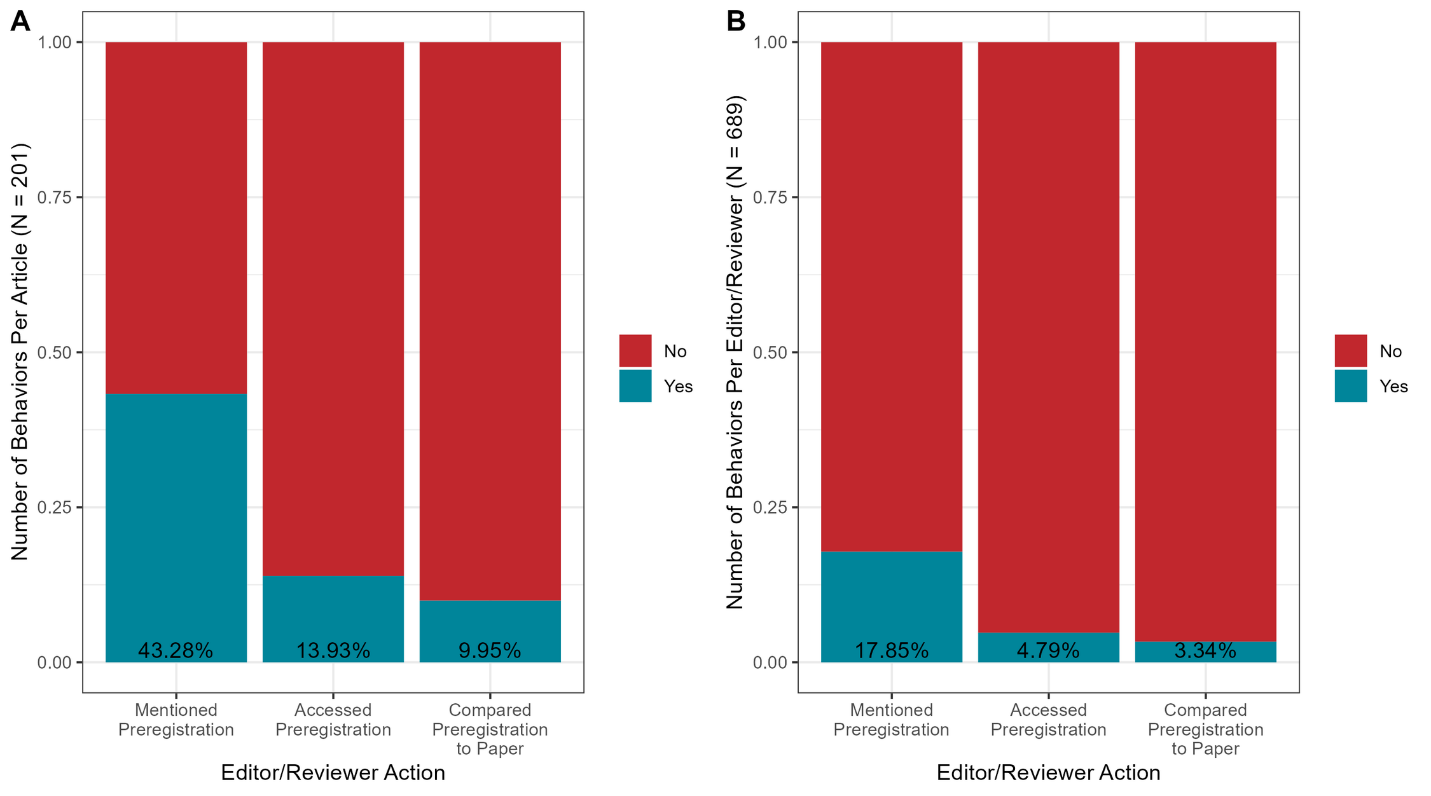
\includegraphics[width=\textwidth]{media/image2.png}

		\caption{\textbf{Frequencies of Reported Preregistration Checking Behavior.}\emph{ }Summary of frequencies in which editors/reviewers mentioned preregistration, indicate accessing the preregistration, and compared the preregistration plan to the reporting in the manuscript. Panel A shows data for the article level (\emph{n} = 201) and Panel B for the editor/reviewer level (\emph{n} = 689). Accessible color palette selected using\url{https://venngage.com/tools/accessible-color-palette-generator.}}

		\label{fig:rId11}


	\end{figure*}

	\subsection{How often do editors and reviewers report on the relation between the preregistration plans and reporting in the article? When they do, what do they highlight?}



	In 10\% of articles (\emph{n} = 20) at least one editor/reviewer discussed the relation between the preregistration and the manuscript (one person: \emph{n} = 17, 8.5\%; two people: \emph{n} = 3, 1.5\%), but this frequency dropped to just 3\% when looking at the editor/reviewer level.



	Of the small number (\emph{n} = 22) of reviewers who commented on the relation between the preregistration and the manuscript, most (\emph{n} = 16) noted some level of undisclosed deviations. Most of these comments highlighted a variety of undisclosed deviations (\emph{n} = 12), with others specifically indicating registered analyses that were not reported in the paper at all (\emph{n} = 2), registered models being different in the preregistration and the paper (\emph{n} = 1), and authors not disclosing that some of the data were collected prior to the registration (\emph{n} = 1). The six comments not directly about deviations include noting that the preregistration contained clearer rationale than the paper, different hypothesis numbering in the two documents, and questions about the date of registration relative to data collection (\emph{n} = 2; the sixth comment constituted a reviewer who initially commented about undisclosed deviations, but in a later round of review acknowledged that they were mistaken). Only one of the 22 reviewers who checked the preregistration commented that the authors had adhered to their plan.



	Comparing the frequencies of engagement with preregistration between editors and reviewers was not part of the preregistration plan, but worth noting here because of just how stark the difference was. Only 20 editors (10\%) mentioned the preregistration and only two editors indicated accessing the preregistration, both of which compared the relation between the preregistration and the manuscript. This is an extremely low level of engagement with preregistrations by editors.



	\subsection{Are there any variations in the preceding by discipline, journal, or research topic?}



	As noted in the preregistration, the degree to which variations by discipline, journal, or research topic could be examined would depend on the frequencies found in the preceding. Given the very low frequencies, especially at the editor/reviewer level of analysis, I decided not to conduct these analyses as I do not believe that any meaningful conclusions could be drawn. The data are openly available at \url{https://osf.io/nmhbf/}, so those interested in doing so may conduct their own analysis.



	\section{\textbf{Discussion}}



	The results of the present study indicate an extremely low rate of editors and reviewers engaging with preregistration plans during the review process—much lower than the self-reported rates of engagement (Mathieu, 2009; Willroth \& Atherton, 2024). The rates are low when looking at the article level, that is, whether any editor/reviewer engaged with the preregistration for a given manuscript, but the data are particularly grim when looking at the reviewer level, indicating that overall reported engagement with preregistrations during the review process is scarce.



	At the paper level, there was a decent frequency of comments about the preregistration, which were either positive or neutral. The frequency of accessing the preregistration dropped markedly, indicating that even when recognizing that a study was preregistered, editors/reviewers do not meaningfully engage with it. Again, the situation looks much worse at the editor/reviewer level. Moreover, on the rare occasions when reviewers \emph{do} report examining the preregistrations in relation to the manuscripts, they tend to discover undisclosed deviations.



	It is clear that editors and reviewers need to improve the rigor of their reviews and evaluate preregistration plans as part of the review process. A common objection to this mandate is that this is a lot to ask of reviewers, who are already over-burdened. Evaluating preregistration plans would simply take too much time. As a seasoned editor and reviewer, I would argue back that reviewers currently do not use their time efficiently. Indeed, I will unapologetically state that they often waste time highlighting typos and grammatical errors, or generating long-winded grievances about omitted literatures or “lack of theory.” This is not time well spent. Peer review is most productive when it focuses on the technical merits of a study, and evaluating preregistration plans is absolutely part of that. Additionally, it is certainly the case that some editors and reviewers are unfamiliar with what preregistrations are and how they should evaluate them, whereas others may even be opposed to the practice altogether. Both situations would lead to lack of engagement with the preregistration plans, albeit for different reasons. The suggestions and template provided by Willroth and Atherton (2024) supplies researchers from all backgrounds and perspectives with strong rationale for why the plans should be checked, as well as concrete tools that authors and reviewers can put into action.



	It is also clear that researchers need to improve their studies and reporting. First, authors could work to develop stronger and clearer preregistration plans. Both Bakker et al. (2020) and Willroth and Atherton (2024) are excellent resources for supporting this goal, and I urge all readers to consult them. Despite the need to do better, it is important to note that a preregistration will rarely be perfect. Even with the current paper, which is focused on preregistration transparency, some questions about the relation between the preregistration and the manuscript arose during review. The transparency facilitated by the existence of the preregistration, along with a reviewer who engaged with it, led to a stronger paper. Second, if authors were clearer and more transparent in their reporting, it would reduce the effort and time investment required of the reviewers. Researchers preregister their work presumably because they see some value in doing so. That value, however, is not realized without transparent reporting of what exactly was preregistered and if there were any deviations (see Willroth \& Atherton, 2024). As an editor, reviewer, and collaborator, I often advocate for what I will now call the “eight-word solution,” inspired by the 21-word solution (Simmons et al., 2012). Towards the beginning of the Results section, authors should include the following statement: “All reported analyses were preregistered unless otherwise specified,” and then they should ensure that the statement is true. The value of this statement is that it is an active proclamation, and thus any violations of the statement would be a clear case of scientific dishonesty. I am not so naïve as to expect that simply adding this statement would solve all of the problems, but it does represent an improvement over the vast sea of vagary currently observed in studies claiming to be preregistered.



	And, of course, it is clear that journal publishers need to improve their evaluation guidelines and protocols to include review of preregistration and evaluation of the relationships between the preregistered plan and the study manuscript. Publishers, professional societies, and other organizations that produce and oversee journal operations can play a key role in supporting the goals of preregistration. Doing so starts with identifying transparency—the underlying principle of preregistration—as a core value of the journal, and then recruiting editors whose priorities align with that goal. But, as noted, evaluating preregistration plans takes time, and until there is major cultural change within the sciences, we are unlikely to see a rapid increase in the rate of engagement with preregistrations. Journals can and should support an editorial position focused on transparency, openness, and rigor (and this position should be paid for by any journal that collects revenue). For example, the journal \emph{Psychological Science} recently announced a Senior Statistics, Transparency, and Rigor Editor and editorial team, whose job will be to conduct verification checks and ensure computational reproducibility of accepted manuscripts (Hardwicke \& Vazire, 2023). In a separate initiative, the \emph{discrepancy review} intervention has provided initial evidence that having reviewers whose dedicated role is to evaluate preregistration plans in relation to the reporting in the manuscript leads to an effective outcome appreciated by both editors and reviewers (TARG Meta-Research Group and Collaborators, 2022).



	\subsection{Limitations and constraints on generality}



	Importantly, the frequencies reported here should not be considered generalizable estimates of editor/reviewer behavior for several reasons. First, all of the articles were taken from the \emph{PLOS} family of journals, and the vast majority came from \emph{PLOS ONE}. One might argue that the reviews for these articles might have been particularly bad, especially if one has had negative experiences with open-access mega-journals. The benefit of me going through the reviews manually is that I have a sense for what they look like, and although I have no quantified evidence to support my claim, the reviews are no different from the quality I have observed through editing and reviewing thousands of manuscripts.



	Second, the analysis was restricted to accepted articles, so it remains possible that heavy reviewer scrutiny leads to higher rejection rates. Analysis of all submitted and reviewed manuscripts, not just those that were accepted, is certainly needed, although very few journals provide the review history for rejected manuscripts.



	Third, the study was based only on what editors/reviewers reported in their reviews. It is entirely possible that some editors/reviewers do not mention the preregistration if everything checks out, which would then suggest that the current results are biased towards reviewers detecting undisclosed deviations. Clearly some people do this, but there are good reasons to suspect that it is not very frequent: a) the documented rates of high deviations, b) the widespread view that reviewing preregistrations is too burdensome and time-consuming, c) the general lack of knowledge about preregistrations and what they are for, and d) of the many preregistered papers that I have edited/reviewed, only once was there no undisclosed deviations in the paper, and in every decision/review I was the only person who even mentioned the preregistration in the process. None of this is clear evidence, of course, but it does suggest to me that the rate is low. Moving forward, I strongly encourage editors/reviewers to mention that they checked the preregistration in their reviews, as doing so signals to authors and other reviewers/editors that it is important to have a clear connection between the plan and the manuscript, and that checking this is something that reviewers are doing.



	Fourth, the \emph{PLOS} search tool used for the article retrieval process clearly has limits. I know this, because my own preregistered paper published in \emph{PLOS ONE} (Delker et al., 2020) was not included in the search results, despite “pre-registration” appearing in the target fields. Surely, additional eligible articles were missed in the search process. That said, there is no reason to believe that the limitations of the search process led to bias in the results one way or another (for Delker et al., 2020, neither the editors nor the two reviewers mentioned the preregistration in their reviews). Again, the results of this analysis are not meant to serve as generalizable population estimates of editor/reviewer behavior, but rather an initial investigation into how often, and in what way, editors/reviewers engaged with preregistrations during the review process.



	\section{\textbf{Conclusions}}



	If a study is preregistered, but nobody checks it during review, does it mean anything? What is the value of a preregistered article when the preregistration was not actually evaluated during the review process? Very little, I would argue. One of the primary rationales of preregistration is to reduce the prevalence of questionable research practices, hypothesizing after the results are known (HARKing), and undisclosed analytic flexibility (Nosek et al., 2018), but this can only be achieved if those evaluating the manuscript evaluate its consistency with the preregistration plan. If reviewers do not examine the preregistration plans, will the casual reader? Current data suggest no, see Spitzer \& Mueller (2023). Or, will most see that the study was preregistered, either from a badge or from the text, and assign greater rigor to the study and credibility of the findings? Current data suggest yes, see Schneider et al. (2022). If we are going to argue for the value of preregistration we must also argue for the need for them to be evaluated during the review process. Otherwise, they have no meaning at all.



	\section{\textbf{Acknowledgments}}



	Thanks to Amy Riegelman for assistance with the article search and extraction, to Dulce Wilkinson Westberg, Linh Nguyen, and Edward Chou for their help with article coding, and to Emily Willroth, Olivia Atherton, and Veronica Boyce for helpful comments on a previous version. Double recognition to Linh Nguyen for conducting the code review and help with Figure 2. I alone am responsible for the contents and all errors reported in this manuscript. Data, code, materials, supplements, and preregistration: \url{https://osf.io/nmhbf/}.







	\section{References:}


	\indent Bakker, M., Veldkamp, C. L. S., van Assen, M. A. L. M., Crompvoets, E. A. V., Ong, H. H., Nosek, B. A., Soderberg, C. K., Mellor, D., \& Wicherts, J. M. (2020). Ensuring the quality and specificity of preregistrations. \emph{PLOS Biology}, \emph{18}(12), Article e3000937. \url{https://doi.org/10.1371/journal.pbio.3000937}



	Chambers, C. D., \& Tzavella, L. (2021). The past, present and future of Registered Reports. \emph{Nature Human Behaviour}, \emph{6}, 29-42. \url{https://doi.org/10.1038/s41562-021-01193-7}



	Claesen, A., Gomes, S., Tuerlinckx, F., \& Vanpaemel, W. (2021). Comparing dream to reality: An assessment of adherence of the first generation of preregistered studies. \emph{Royal Society Open Science}, \emph{8}(10), Article 211037. \url{https://doi.org/10.1098/rsos.211037}



	Comtois, D. (2022). \emph{summarytools: Tools to Quickly and Neatly Summarize Data} [Computer software]. R package version 1.0.1.



	Conix, S., Cuypers, V., Zachos, F. E., Artois, T., \& Monnens, M. (2023). A plea for preregistration in taxonomy. \emph{Megataxa}, \emph{10}(1), 1-14. \url{https://doi.org/10.11646/megataxa.10.1.1}



	Delker, B. C., Salton, R., McLean, K. C., \& Syed, M. (2020). Who has to tell their trauma story and how hard will it be? Influence of cultural stigma and narrative redemption on the storying of sexual violence. \emph{PLOS ONE}, \emph{15}(6), Article e0234201. \url{https://doi.org/10.1371/journal.pone.0234201}



	Dirnagl, U. (2020). Preregistration of exploratory research: Learning from the golden age of discovery. \emph{PLOS Biology}, \emph{18}(3), Article e3000690. \url{https://doi.org/10.1371/journal.pbio.3000690}



	Errington, T. M., Mathur, M., Soderberg, C. K., Denis, A., Perfito, N., Iorns, E., \& Nosek, B. A. (2021). Investigating the replicability of preclinical cancer biology. \emph{eLife}, \emph{10}, Article e71601. \url{https://doi.org/10.7554/eLife.71601}



	Haddaway, N. R., Page, M. J., Pritchard, C. C., \& McGuinness, L. A. (2022). \emph{PRISMA2020}: An R package and Shiny app for producing PRISMA 2020-compliant flow diagrams, with interactivity for optimised digital transparency and Open Synthesis. \emph{Campbell Systematic Reviews}, \emph{18}(2), Article e1230. \url{https://doi.org/10.1002/cl2.1230}



	Hardwicke, T. E., \& Vazire, S. (2023). Transparency is now the default at psychological science. \emph{Psychological Science}, \emph{35}(7), 708-711. \url{https://doi.org/10.1177/09567976231221573}



	Haven, T. L., \& Van Grootel, L. (2019). Preregistering qualitative research. \emph{Accountability in Research}, \emph{26}(3), 229--244. \url{https://doi.org/10.1080/08989621.2019.1580147}



	Kampman, J. M., Turgman, O., Sperna Weiland, N. H., Hollmann, M. W., Repping, S., \& Hermanides, J. (2022). Statistical robustness of RCTs in high-impact journals has improved, but was low across medical specialties. \emph{Journal of Clinical Epidemiology}, \emph{150}, 165-170. \url{https://doi.org/10.1016/j.jclinepi.2022.07.001}



	Kidwell, M. C., Lazarević, L. B., Baranski, E., Hardwicke, T. E., Piechowski, S., Falkenberg, L.-S., Kennett, C., Slowik, A., Sonnleitner, C., Hess-Holden, C., Errington, T. M., Fiedler, S., \& Nosek, B. A. (2016). Badges to acknowledge open practices: A simple, low-cost, effective method for increasing transparency. \emph{PLOS Biology}, \emph{14}(5), e1002456. \url{https://doi.org/10.1371/journal.pbio.1002456}



	Lakens, D. (2019). The value of preregistration for psychological science: A conceptual analysis. \emph{Japanese Psychological Review, 62}(3), 221-230. \url{https://doi.org/10.24602/sjpr.62.3_221}



	Lakens, D. (2024). When and how to deviate from a preregistration. \emph{Collabra: Psychology}, \emph{10}(1), Article 117094. \url{https://doi.org/10.1525/collabra.117094}



	Mathieu, S. (2009). Comparison of registered and published primary outcomes in randomized controlled trials. \emph{JAMA}, \emph{302}(9), 977-984. \url{https://doi.org/10.1001/jama.2009.1242}



	Nosek, B. A., Ebersole, C. R., DeHaven, A. C., \& Mellor, D. T. (2018). The preregistration revolution. \emph{Proceedings of the National Academy of Sciences}, \emph{115}(11), 2600--2606. \url{https://doi.org/10.1073/pnas.1708274114}



	Pariente, N. (2022). Premiering pre-registration at PLOS Biology. \emph{PLOS Biology}, \emph{20}(3), Article e3001611. \url{https://doi.org/10.1371/journal.pbio.3001611}



	Posit Team. (2023). \emph{Rstudio: Integrated development environment for R} [Computer software]. Posit Software, PBC. \url{http://www.posit.co/}



	Quintana, D. S. (2015). From pre-registration to publication: A non-technical primer for conducting a meta-analysis to synthesize correlational data. \emph{Frontiers in Psychology}, \emph{6}, Article 1549. \url{https://doi.org/10.3389/fpsyg.2015.01549}



	R Core Team. (2022). \emph{R: A language and environment for statistical computing} [Computer software]. R Foundation for Statistical Computing. \url{https://www.R-project.org/}



	Rubin, M., \& Donkin, C. (2022). Exploratory hypothesis tests can be more compelling than confirmatory hypothesis tests. \emph{Philosophical Psychology}, 37(8), 2019-2047. \url{https://doi.org/10.1080/09515089.2022.2113771}



	Schneider, J., Rosman, T., Kelava, A., \& Merk, S. (2022). Do open-science badges increase trust in scientists among undergraduates, scientists, and the public? \emph{Psychological Science}, \emph{33}(9), 1588--1604. \url{https://doi.org/10.1177/09567976221097499}



	Simmons, J. P., Nelson, L. D., \& Simonsohn, U. (2012). \emph{A 21 Word Solution} (SSRN Scholarly Paper No. 2160588). \url{https://doi.org/10.2139/ssrn.2160588}



	Spitzer, L., \& Mueller, S. (2023). Registered report: Survey on attitudes and experiences regarding preregistration in psychological research. \emph{PLOS ONE}, \emph{18}(3), Article e0281086. \url{https://doi.org/10.1371/journal.pone.0281086}



	Syed, M. (2024). Three persistent myths about open science. \emph{Journal of Trial and Error}, \emph{4}(2). \url{https://doi.org/10.36850/mr11}



	Syed, M., \& Nelson, S. C. (2015). Guidelines for establishing reliability when coding narrative data. \emph{Emerging Adulthood}, \emph{3}(6), 375--387. \url{https://doi.org/10.1177/2167696815587648}



	Szollosi, A., Kellen, D., Navarro, D. J., Shiffrin, R., van Rooij, I., Van Zandt, T., \& Donkin, C. (2020). Is preregistration worthwhile? \emph{Trends in Cognitive Sciences}, \emph{24}(2), 94--95. \url{https://doi.org/10.1016/j.tics.2019.11.009}



	TARG Meta-Research Group and Collaborators. (2022). Discrepancy review: A feasibility study of a novel peer review intervention to reduce undisclosed discrepancies between registrations and publications. \emph{Royal Society Open Science}, \emph{9}(7), Article 220142. \url{https://doi.org/10.1098/rsos.220142}



	Thibault, R. T., Pennington, C. R., \& Munafò, M. R. (2023). Reflections on preregistration: Core criteria, badges, complementary workflows. \emph{Journal of Trial and Error}, \emph{4}(1). \url{https://doi.org/10.36850/mr6}



	van den Akker, O. R., van Assen, M. A. L. M., Enting, M., de Jonge, M., Ong, H. H., Rüffer, F., Schoenmakers, M., Stoevenbelt, A. H., Wicherts, J. M., \& Bakker, M. (2023). Selective hypothesis reporting in psychology: Comparing preregistrations and corresponding publications. \emph{Advances in Methods and Practices in Psychological Science}, \emph{6}(3). \url{https://doi.org/10.1177/25152459231187988}



	van den Akker, O. R., Weston, S., Campbell, L., Chopik, B., Damian, R., Davis-Kean, P., Hall, A., Kosie, J., Kruse, E., Olsen, J., Ritchie, S., Valentine, K. D., van 't Veer, A., \& Bakker, M. (2021). Preregistration of secondary data analysis: A template and tutorial. \emph{Meta-Psychology}, \emph{5}. \url{https://doi.org/10.15626/MP.2020.2625}



	van 't Veer, A. E., \& Giner-Sorolla, R. (2016). Pre-registration in social psychology—A discussion and suggested template. \emph{Journal of Experimental Social Psychology}, \emph{67}, 2--12. \url{https://doi.org/10.1016/j.jesp.2016.03.004}



	Vazire, S. (2017). Quality Uncertainty Erodes Trust in Science. \emph{Collabra: Psychology}, \emph{3}(1), Article 1. \url{https://doi.org/10.1525/collabra.74}



	Wagenmakers, E.-J., Wetzels, R., Borsboom, D., van der Maas, H. L. J., \& Kievit, R. A. (2012). An agenda for purely confirmatory research. \emph{Perspectives on Psychological Science}, \emph{7}(6), 632--638. \url{https://doi.org/10.1177/1745691612463078}



	Wickham, H. (2016). \emph{ggplot2: Elegant Graphics for Data Analysis} [Computer software].



	Wickham, H., François, R., Henry, L., Müller, K., \& Vaughan, D. (2023). \emph{dplyr: A grammar of data manipulation} (Version R package version 1.1.3) [Computer software]. \url{https://CRAN.R-project.org/package=dplyr}



	Wickham, H., Vaughan, D., \& Girlich, M. (2023). \emph{tidyr: Tidy messy data} (Version R package version 1.3.0) [Computer software]. \url{https://CRAN.R-project.org/package=tidyr}



	Wilke, C. O. (2020). \emph{cowplot: Streamlined Plot Theme and Plot Annotations for “ggplot2”} [Computer software]. R package version 1.1.1. \url{https://CRAN.R-project.org/package=cowplot}



	Willroth, E. C., \& Atherton, O. E. (2024). Best laid plans: A guide to reporting preregistration deviations. \emph{Advances in Methods and Practices in Psychological Science}, \emph{7}(1). \url{https://doi.org/10.1177/25152459231213802}











	\section{\textbf{Supporting information}}







	S1 Table. Keywords for Articles Included in Analysis (Full List)


\end{document}